\let\negmedspace\undefined
\let\negthickspace\undefined
\documentclass[journal]{IEEEtran}
\usepackage[a5paper, margin=10mm, onecolumn]{geometry}
\usepackage{lmodern} % Ensure lmodern is loaded for pdflatex
\usepackage{tfrupee} % Include tfrupee package

\setlength{\headheight}{1cm} % Set the height of the header box
\setlength{\headsep}{0mm}     % Set the distance between the header box and the top of the text

\usepackage{gvv-book}
\usepackage{gvv}
\usepackage{cite}
\usepackage{amsmath,amssymb,amsfonts,amsthm}
\usepackage{algorithmic}
\usepackage{graphicx}
\usepackage{textcomp}
\usepackage{xcolor}
\usepackage{txfonts}
\usepackage{listings}
\usepackage{enumitem}
\usepackage{mathtools}
\usepackage{gensymb}
\usepackage{comment}
\usepackage[breaklinks=true]{hyperref}
\usepackage{tkz-euclide} 
\usepackage{listings}                                      
\def\inputGnumericTable{}                                 
\usepackage[latin1]{inputenc}                                
\usepackage{color}                                            
\usepackage{array}                                            
\usepackage{longtable}
\usepackage{multicol}
\usepackage{calc}                                             
\usepackage{multirow}                                         
\usepackage{hhline}                                           
\usepackage{ifthen}                                           
\usepackage{lscape}
\begin{document}

\bibliographystyle{IEEEtran}
\vspace{3cm}

\title{10.3.2.2.1}
\author{EE24BTECH11006 - Arnav Mahishi}
% \maketitle
% \newpage
% \bigskip
{\let\newpage\relax\maketitle}

\renewcommand{\thefigure}{\theenumi}
\renewcommand{\thetable}{\theenumi}
\setlength{\intextsep}{10pt} % Space between text and floats


\numberwithin{equation}{enumi}
\numberwithin{figure}{enumi}
\renewcommand{\thetable}{\theenumi}


\textbf{Question}:\newline
Find out whether the lines $5x-4y+8=0$ and $7x+6y-9=0$ intersect at a point, parallel or coincident 
\newline
\begin{table}[h!]    
  \centering
  \begin{tabular}[12pt]{ |c| c| c |}
    \hline
    \textbf{Variable} & \textbf{Description} & \textbf{values}\\ 
    \hline
    $\vec{V}$ & Quadratic form of the matrix & $\myvec{1 & 0 \\ 0 & 1} $\\
    \hline
    $\vec{u}$ & Linear coefficient vector & $\myvec{0 \\ 0} $\\
    \hline
    f & constant term & -4 \\ 
    \hline
    $\vec{m}$ & The direction vector of line & $\myvec{1 \\ 0}$\\
    \hline
     $\vec{h}$ & Point on line & \myvec{2 \\ 0} \\
     \hline
\end{tabular}

  \caption{Variables Used}
  \label{tab1.1.2.2}
\end{table}
\newline
\textbf{Theoretical Solution:}\\
Let $a_1$,$b_1$, and $c_1$ and $a_2$,$b_2$, and $c_2$ be the coefficents of $x$,$y$, and $1$ in lines $1$ and $2$ respectively.\\
We get:
\begin{align}
    \frac{a_1}{a_2}=\frac{5}{7}\\
    \frac{b_1}{b_2}=\frac{-2}{3}\\
    \frac{c_1}{c_2}=\frac{-8}{9}\\
    m_1=\frac{-a_1}{b_1}=\frac{5}{4}\\
    m_2=\frac{-a_2}{b_2}=\frac{7}{6}
\end{align}
As all the ratios aren't equal to each other neither are $m_1$ and $m_2$ equal\\
$\therefore$ The lines intersect at a point\\
\textbf{Computational Solution:}\\
The set of linear equations $5x-4y+8=0$ and $7x+6y-9=0$ can be represented by the following equation
\begin{align}
    \myvec{5&-4\\7&6}\myvec{x\\y}=\myvec{-8\\9}
\end{align}
Any non-singular matrix can be represented as a product of a lower triangular matrix $L$ and an
upper triangular matrix $U$:
\begin{align}
    A = L \cdot U
\end{align}
1. Initialization: 
   - Start by initializing $ \mathbf{L} $ as the identity matrix $ \mathbf{L} = \mathbf{I} $ and $ \mathbf{U} $ as a copy of $ \mathbf{A} $.
   
2. Iterative Update:
   - For each pivot $ k = 1, 2, \ldots, n $:
     - Compute the entries of $ U $ using the first update equation.
     - Compute the entries of $ L $ using the second update equation.
   
3. Result:
   - After completing the iterations, the matrix $ \mathbf{A} $ is decomposed into $ \mathbf{L} \cdot \mathbf{U} $, where $ \mathbf{L} $ is a lower triangular matrix with ones on the diagonal, and $ \mathbf{U} $ is an upper triangular matrix.
\subsection*{1. Update for $ U_{k,j} $ (Entries of $ U $)}

For each column $ j \geq k $, the entries of $ U $ in the $ k $-th row are updated as:
\[
U_{k,j} = A_{k,j} - \sum_{m=1}^{k-1} L_{k,m} \cdot U_{m,j}, \quad \text{for } j \geq k.
\]
This equation computes the elements of the upper triangular matrix $ \mathbf{U} $ by eliminating the lower triangular portion of the matrix.

\subsection*{2. Update for $ L_{i,k} $ (Entries of $ L $)}

For each row $ i > k $, the entries of $ L $ in the $ k $-th column are updated as:
\[
L_{i,k} = \frac{1}{U_{k,k}} \left( A_{i,k} - \sum_{m=1}^{k-1} L_{i,m} \cdot U_{m,k} \right), \quad \text{for } i > k.
\]
This equation computes the elements of the lower triangular matrix $ \mathbf{L} $, where each entry in the column is determined by the values in the rows above it.\\
Using a code we get L,U as 

\textbf{Step-by-Step Process:}\\

\textbf{1. Initial Matrix:}
\begin{align}
    A = \myvec{5 & -4 \\ 7 & 6}
\end{align}

\textbf{2. Compute $U$ (Upper Triangular Matrix):}\\
Using the update equation for $U$:
\begin{align}
    U_{11} = A_{11} = 5, \quad U_{12} = A_{12} = -4
\end{align}
For $U_{22}$:
\begin{align}
    U_{22} = A_{22} - L_{21} \cdot U_{12} = 6 - \frac{7}{5} \cdot (-4) = \frac{58}{5}
\end{align}

\textbf{3. Compute $L$ (Lower Triangular Matrix):}\\
Using the update equation for $L$:
\begin{align}
    L_{21} = \frac{A_{21}}{U_{11}} = \frac{7}{5}
\end{align}
The final $L$ matrix is:
\begin{align}
    L = \myvec{1 & 0 \\ \frac{7}{5} & 1}
\end{align}

\textbf{4. Solving the System:}\\
Using the equations $L\vec{y} = \vec{b}$ and $U\vec{x} = \vec{y}$:
\begin{itemize}
    \item \textbf{Forward Substitution:}
    \begin{align}
        \myvec{1 & 0 \\ \frac{7}{5} & 1}\myvec{y_1 \\ y_2} = \myvec{-8 \\ 9}
    \end{align}
    Solving gives:
    \begin{align}
        y_1 = -8, \quad y_2 = \frac{101}{5}
    \end{align}

    \item \textbf{Backward Substitution:}
    \begin{align}
        \myvec{5 & -4 \\ 0 & \frac{58}{5}}\myvec{x_1 \\ x_2} = \myvec{-8 \\ \frac{101}{5}}
    \end{align}
    Solving gives:
    \begin{align}
        x_2 = \frac{101}{58}, \quad x_1 = \frac{-6}{29}
    \end{align}
\end{itemize}

Thus, the solution is:
\begin{align}
    \vec{x} = \myvec{\frac{-6}{29} \\ \frac{101}{58}}
\end{align}

\begin{figure}[h!]
   \centering
   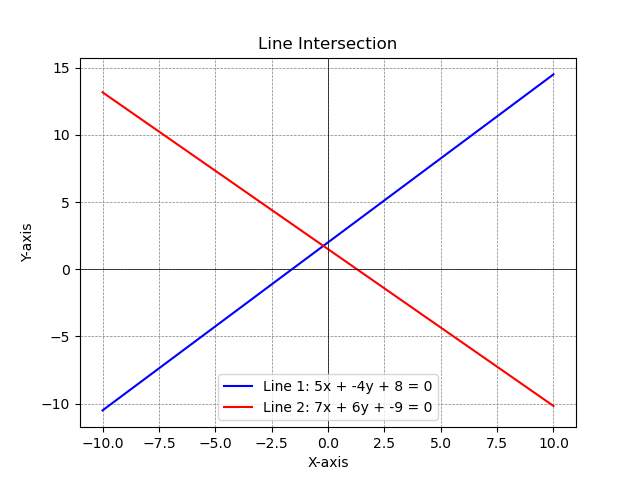
\includegraphics[width=0.7\columnwidth]{figs/fig.png}
    \caption{Solution to set of linear equations}
\end{figure}
\end{document}

